%------------------------------------------------------------------------------
%    project: 'ss_1'
%
%    authors: Simone Santoni (simone.snatoni.1@city.ac.uk) and
%             Jost Sieweke (j.sieweke@vu.nl)
%
%    dates: created Thu  9 Jan 15:33:28 2020
%           last change --
% -----------------------------------------------------------------------------

\documentclass[11pt, english]{article}


% -----------------------------------------------------------------------------
% packages
% -----------------------------------------------------------------------------

% page and paragraph layout
% -------------------------
\usepackage[a4paper]{geometry}
\geometry{verbose,tmargin=1in,bmargin=1in,lmargin=1in,rmargin=1in}
%\setcounter{secnumdepth}{-2}
%\setcounter{tocdepth}{-2}
\usepackage{setspace}
\onehalfspacing%\doublespacing
\setlength{\parindent}{2.75em}
\setlength{\parskip}{1em}
%\renewcommand{\baselinestretch}{1.5}
\usepackage{titlesec}
\titlespacing{\section}{0pt}{1.5ex}{-1.5ex}
\titlespacing{\subsection}{0pt}{1.5ex}{-1.5ex}
\titlespacing{\subsubsection}{0pt}{1.5ex}{-1.5ex}

% text style
% ----------
\usepackage{color}

% links
% -----
\usepackage{hyperref}

% paragraphs
% ----------
%\makeatletter
%\renewcommand{\@seccntformat}[1]{}
%\makeatother

% endnote
% -------
\usepackage{endnotes}
%\let\footnote=\endnote

% bibliography
% ------------
\usepackage[
%natbib=true,
backend=biber,
%style=alphabetic,
citestyle=authoryear,
%hyperref=true,
%maxbibnames=99,
%firstinits=false
%maxcitenames=4,
%citetracker=true,
%parentracker=true,
bibstyle=authortitle,
]{biblatex}

% exhibits
% --------
\usepackage{dcolumn}
\usepackage{tabularx,ragged2e}
\usepackage{threeparttable}
\usepackage{graphicx}
\usepackage{rotating}
%\usepackage[T1]{fontenc}
%\usepackage{times}
%\usepackage{amsmath}
%\usepackage{mathptmx}
%\usepackage{bbm}
%\usepackage{dsfont}
\usepackage{array,booktabs}
\usepackage{etoolbox}
\usepackage{caption}
\captionsetup[table]{labelfont=sc, labelsep=newline}
\captionsetup[figure]{labelfont=sc, labelsep=period}
\renewcommand{\figurename}{Fig.}
\usepackage{etoolbox}
\usepackage{ctable}
\renewcommand{\thetable}{\Roman{table}}

% appendices
% ----------
\usepackage{appendix}

% authors
% -------
\usepackage{authblk}


% -----------------------------------------------------------------------------
% load biblio
% -----------------------------------------------------------------------------

\bibliography{references.bib}


% -----------------------------------------------------------------------------
% cover page
% -----------------------------------------------------------------------------

\title{Natural Experiments in Strategic Management Research:\\
       A Review and Guidelines}

\author[1]{\href{simone.santoni.1@city.ac.uk}{Simone Santoni}}
\author[2]{\href{j.sieweke@vu.nl}{Jost Sieweke}}
\affil[1]{Cass Business School --- City, University of London}
\affil[2]{Vrije Universiteit Amsterdam}


%------------------------------------------------------------------------------
% body of the document
% -----------------------------------------------------------------------------
  
\begin{document}

\begin{singlespace}
  
\maketitle

%\begin{abstract}
%
%---Abstract goes here---
%
%\bigskip
%
%\textit{Keywords}: kw1, kw2, kw3.
%
%\end{abstract}

\end{singlespace}

\clearpage


\section{Introduction}
\label{sec:introduction}

% recall causal inference issues, mention attempts made by the community
% to improve causal inference, and connect these efforts with the popularity
% of natural experiments

\noindent The quest for empirical identification in strategic management
research has created substantial attention around `natural experiments,' a form
of causal inquiry that has been traditionally popular in economics
\parencite[][]{Meyer1995,Rosenzweig2000} and political science
\parencite[][]{Dunning2008}.  The case for natural experiments is the presence
of `naturally' occurring events---such as new regulations and laws, natural
disasters, or economic and political crises---that heterogeneously influence
the units of a population \parencite[][]{Dunning2012,Robinson2009}. Insofar as
these events generate random or as-if random variations in the environment,
natural experiments mimic the experimental ideal in which units are split into a
treatment and a control group, or, alternatively, receive different levels of
the treatment. Ultimately, this opens up the possibility to infer causal effects
when the substantive relationship at hand is difficult to investigate in a
laboratory setting and/or would require operating costly, impractical, or
unethical field experiments.

% motivation for the article - NEs are not rooted in the field of strategic
% mangagement; rather, they are emerging as one of the most popular ways to
% tackle on the endogeneity challenge. As NEs diffuse in management research,
% pracrices emerge and crystallize on how to discover and leverage exogenous
% variations in order to test causal relationships. 

Despite naturally occurring events can turn into opportunities to conduct causal
research, there are limited guidelines that help strategic management
scholars to prepare and review papers that implement the natural
experiment research design. In order to fill this gap, we highlight the 
strengths and weaknesses of natural experiments as operated in the strategic 
management community and propose actionable suggestions to assess and communicate
the validity of natural experiments.

To do so, we critically review the population of 50 natural experiments
published in the Strategic Management Journal. Particularly, our analysis is
motivated by the following research questions: \emph{R1 --- How do strategy
    scholars claim the random or as-if random nature of environmental variation
    at the core of a natural experiment? R2 --- How do they claim the empirical
    and substantive relevance of a natural experiment? R3 --- How do they claim
    the credibility of the statistical model encapsulated in a natural
experiment design?}

% what we do - we survey papers adopting a NE research design and take stock of
% the emerging practices. Then, we analyze these practices through a validity
% framework (i.e., Dunning's framework) in order to highlight critical
% areas/dimensions along which NE applications can be improved. Finally, we
% provide guidelines that help reviewers and authors in analyzing the validity
% of a NE paper

% contribution of the article - we aim at assisting scholars to get the most out
% of the NE paper and clarify the expectations about what a 'good' quality NE
% paper is (this could smooth the review process)


% organization of the article
This work is organized as follows. The next two sections briefly introduce the key
features of the `standard natural experiment' (i.e., the specific form of
natural experiment considered in this review), along with the evaluative
framework we use to analyze the individual natural experiments. The following
section describes the selection of the reviewed studies. Then, we present the
key insights that stem from our analysis and conclude with a suggested
check-list that facilitates strategy scholars to exploit the opportunities of
causal inference offered by naturally occurring events. The online appendix
contains companion software code to operate natural experiments in Python, R,
and Stata.


\section{Natural Experiments and Causal Empirical Research}
\label{sec:standard_ne}


\subsection{Foundations and Examples from Strategic Management}
\label{sub:foundations_examples}

% we introduce the reader to Dunning's framework 
\noindent The 'standard' natural experiment\footnote{In his comprehensive,
    cross-disciplinary analysis of the literature, Dunning
    \citeyear[][]{Dunning2012} identifies
    three forms of natural experiments: Standard natural experiments;
    instrumental variables (Angrist, 1990); regression discontinuity designs
    (Thistlethwaite \& Campbell, 1960). In the interest of clarity and
    integrity, our review concentrates on standard natural experiments, whose
    origin goes back to the highly acclaimed and impactful research Dr John Snow
    (Snow, 1855) conducted on the diffusion of cholera in the mid
19\textsuperscript{th} century London. In this paper we use the term `natural
experiment' to exclusively refer to standard natural experiments.} resembles the
design of a randomized experiment. In fact, the naturally occurring event (such
as an earthquake, see for example \cite[][]{Belloc2016}) is supposed
to determine the treatment status of the statistical units (treated Vs control),
each of which has both a pre- and a post-treatment observation. As shown in
Figure \ref{fig:ne_logic_viz}, it is possible to estimate the causal effect of the treatment by
contrasting the pre-post change in the outcome variable $y$ across
the control group ($\gamma$) and the treatment group 
($ \gamma + \delta$).

\begin{figure}[]
    \centering
    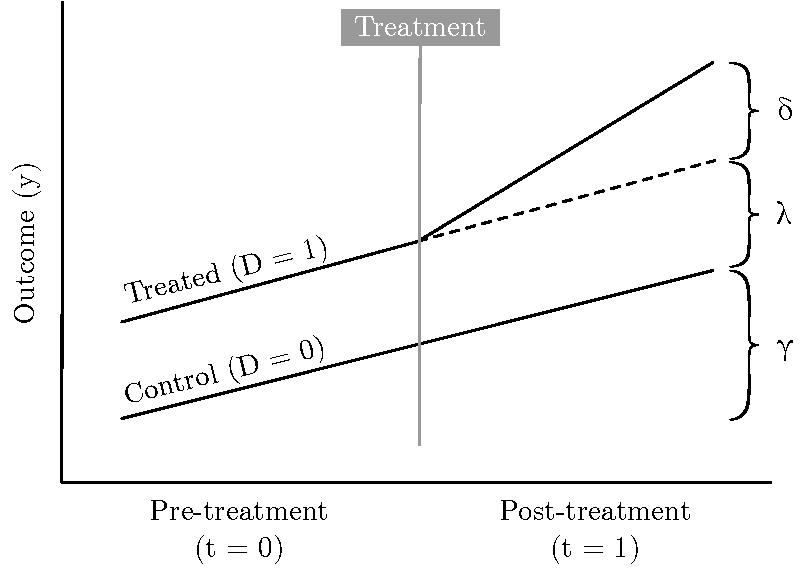
\includegraphics[width=0.62\textwidth]{images/ne_logic_viz.pdf}
    \caption{Visual representation of the standard natural experiment. Notes.---
        The underlying population regression function is $y = \gamma t +
        \lambda D + \delta t D$, where $\gamma$, $\lambda$, and $\delta$ represent 
        the systematic difference in the outcome across the treated and control 
        cases, the trend effect and the difference in the outcome that is due to
        the treatment. For sake of clarity, we represent the case in which
        $\delta > 0$.}
    \label{fig:ne_logic_viz}
\end{figure}

\noindent \textbf{!! Comment: One or two examples of natural experiments
published in SMJ to be succinctly summarized here!!}

\subsection{Assessing the Validity of Natural Experiment Designs}
\label{sub:validity_framework}

\noindent\emph{How do we evaluate a standard natural experiment research
design?} According to Dunning (\cite*[][page 27]{Dunning2012}), the validity of
a natural experiment should be assessed against three criteria (see Figure
\ref{fig:validity_framework}).  First, the authors should prove the random
nature of the treatment, or, at least, defend the plausibility of as-if random.
In the case of the \emph{randomized standard natural experiment}, it is
important that the assignment process is truly random. Although this may seem
obvious, this condition is sometimes violated, even in the context of lotteries
\parencite[e.g.][]{Starr1997}. In the case of an \emph{as-if randomization}, it
is vital the assignment process, although not truly random, is independent of
factors that are related to the outcome and it not affected by unit's
self-selection into treatment or control conditions. As Dunning points out, the
researcher has to make a very compelling case for this assertion (or to drop the
claim to a natural experiment). In depth knowledge of the context (e.g.,
industry regulatory frameworks), qualitative evidence about the naturally
occurring event (e.g., a new law), and quantitative evidence at the event- and
unit-level are oftentimes essential ingredients to defend the plausibility of
as-if random assignment, and, ultimately, to sustain the natural experiment.

Second, the naturally occurring event should reveal the wider
\emph{``theoretical, substantive, and/or policy issues''} \parencite[][page
29]{Dunning2012} that motivate the study. For example, the sudden, premature
death of a star scientist \parencite[][]{Azoulay2010} create the premises for a
natural experiment that quantifies the spill-over effect of collaborating with
academics who are very prominent in the field.

Finally, the statistical model should fit with the characteristics of the
naturally occurring event. In the case of a randomized standard natural
experiment, simplicity and transparency should take precedence in the data
analysis stage. Particularly, the Neyman's potential outcomes framework
\parencite[][]{Splawa1990}, namely, a treated Vs. control mean comparison test,
should be used \emph{prima facie}. At the same time, some statistical
adjustments may be required even in presence of a random (or as-if random)
treatment. For example, the Stable-Unit-Treatment-Value-Assumption (SUTVA) may
be violated insofar as the treatment status of a unit `i' interferes with the
potential outcome of unit `j'. This is a concern Belloc and colleagues
\parencite*[][]{Belloc2016} seem to have in mind when they estimate the impact
of earthquakes on the probability of institutional change at the city-level in
the Middle-Ages northern and central Italy. In fact, both the distribution and
timing of earthquakes are random. However, the probability a control city will
move from autocratic regimes to self-government is also a function of the
information key actors are exposed to, such as the transition choices made by a
treated, neighbor city. In this case, statistical artefacts would be needed to
take into account the correlation of residuals induced by the geographical
proximity of any pair of units.

\begin{figure}[]
    \centering
    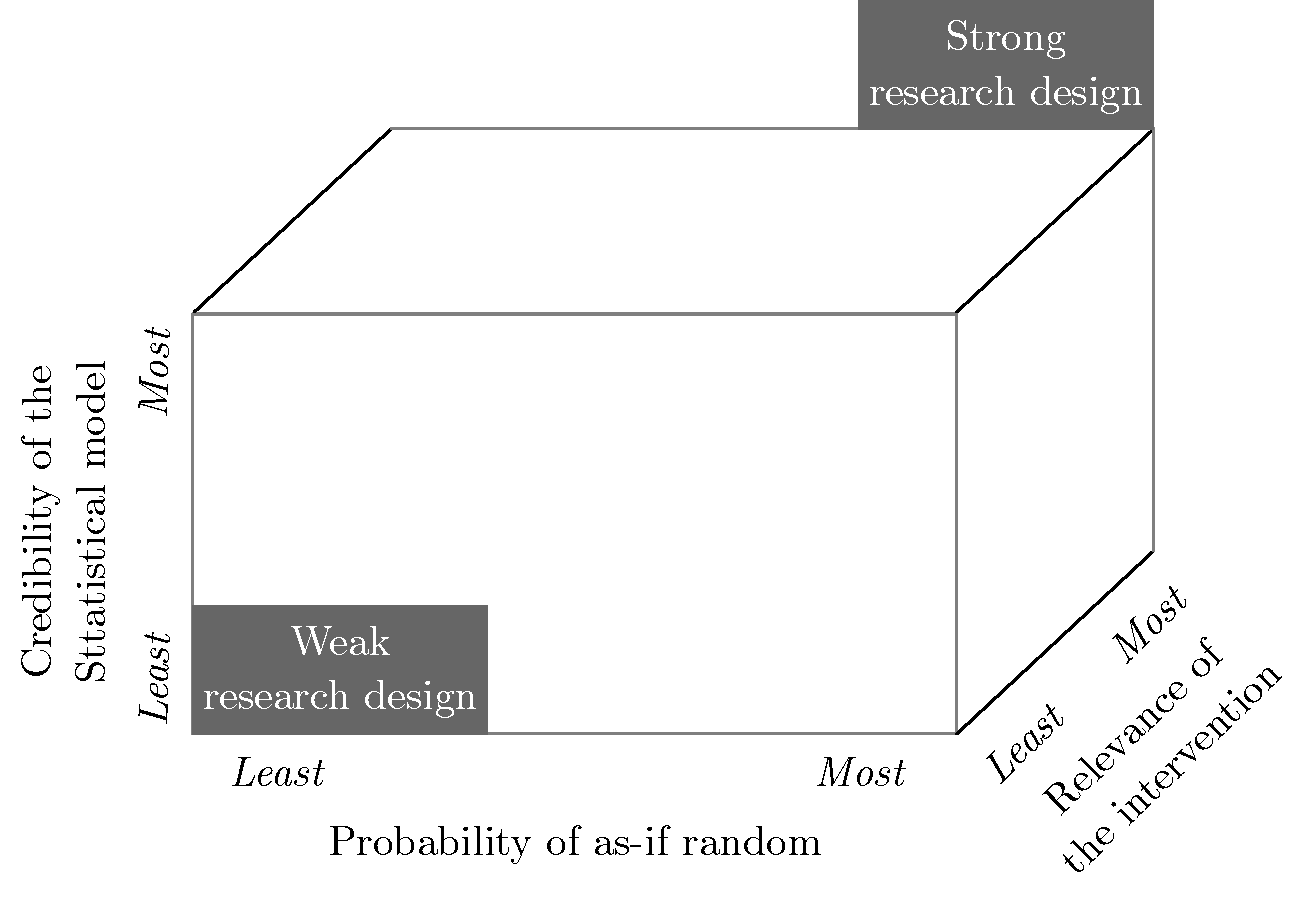
\includegraphics[width=0.78\textwidth]{images/validity_framework.pdf}
    \caption{Visual representation of Dunning's validity framework (Source:
    \cite[][page 31]{Dunning2012})}
    \label{fig:validity_framework}
\end{figure}


\section{Articles Selection}
\label{sec:article_selection}

% data gathering procedure

\noindent  Consistently with previous review of the literature in the field of
strategic management \parencite[e.g.][]{Haans2015}, we decided to survey only
studies published in the Strategic Management Journal.  Using the search engine
available in the journal's web-page, we searched for any article reporting the
quote ``natural experiment*'' in the title, abstract, keywords, \emph{or} full
text of any document published since the very first volume of the journal or
released as pre-print as of December 31, 2019.

We retrieved 73 studies; 50 were eventually included in the review. We excluded
one methodological article \parencite[][]{Semadeni2014}, two articles that
recall the empirical evidence produced in previous natural experiments
\parencite[][]{Gallus2016,Chakrabarti2015}, seven articles that indicate natural
experiments as a possible way to overcome the limitations or expand on the study
at hand \parencite[e.g.][]{Karim2012}, and 13 observational studies
\footnote{Consistently with prior works \parencite[][]{Dunning2012,Sieweke2019},
we use the expression 'observation study' to denote a study oeprating a
correlational research design.} that use the natural experiment label in a
figurative sense to emphasize some appealing properties of the empirical setting
\parencite[][]{Grigoriou2017}. Figure \ref{fig:studies_over_time} illustrates
the distribution of the retrieved studies over time.

\begin{figure}[]
    \centering
    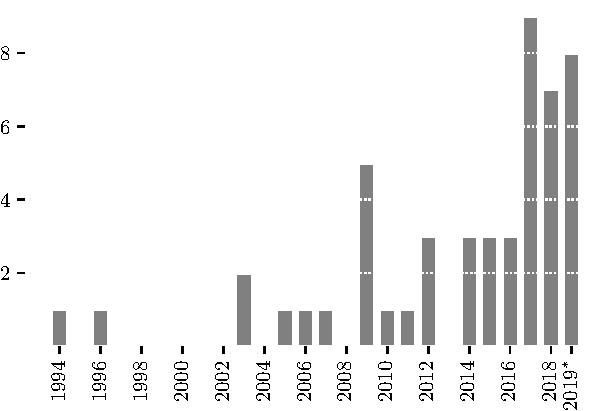
\includegraphics{images/studies_over_time.pdf}
    \caption{Natural experiment studies published in the Strategic Management
        Journal over time. The 2019 bucket, marked with an asterisk, contains 
        both published and accepted, online articles.}
    \label{fig:studies_over_time}
\end{figure}

\section{Assessing the As-If Random Plausibility of the Treatment}

\noindent This section focuses on the diagnostics that can be used to assess and
argument the (as-if) random nature of the environmental variation at the center
of the natural experiment. Specifically, this section surveys and articulates the
following:

\begin{itemize}
    \item diffusion/role of qualitative diagnostics to appreciate:
        \begin{itemize}
            \item units' information about the treatment
            \item units' incentives to self-select into the treatment (control)
                group
            \item unit's capacity to self-select into the treatment (control)
                group
        \end{itemize}
    \item diffusion/role of quantitative diagnostics (e.g., balance test) to 
        compare and contrast treated and control units along relevant dimensions
\end{itemize}

%\subsection{Qualitative Diagnositics}
%
%
%\subsubsection{Units' Information about the Treatment}
%
%.
%
%
%\subsubsection{Units' Incentives to Selef-Select into the Treatment Status}
%
%.
%
%
%\subsubsection{Units' Capacity to Self-Select into the Treatment Status}
%
%.
%
%
%\subsection{Quantitative Diagnostics---Balance Test}
%
%.
%

\section{Assessing the Relevance of the Treatment}

\noindent This section focuses on the empirical and substantive relevance of the
environmental variation at the center of a natural experiment.  Particularly,
this section reviews and discusses the following:

\begin{itemize}
    \item diffusion/role of qualitative diagnostics to show:
        \begin{itemize}
            \item the empirical, substantive, and policy relevance of the
                natural experiment
            \item the external validity (non idiosyncrasy) of the natural
                experiment
            \item exclusion of `bundling of treatments' (i.e., environmental
                variations affecting the outcome through multiple causal
                pathways)
        \end{itemize}
    \item diffusion/role of placebo tests supporting the magnitude of the
        average treatment estimation on the treated  (ATT)
    \item diffusion/role of local average treatment estimation (LATE) 
        considerations
\end{itemize}

%\subsection{Idiosincray of Interventions}
%
%
%
%\subsection{Bundling of Treatments}
%
%.
%
%
%\subsection{Placebo Test}
%
%.
%
%
%\subsection{LATE Considerations}
%
%.
%

\section{Assessing the Credibility of the Statistical Model}

\noindent This section focuses on the credibility of the statistical model
encapsulated in the natural experiment design. Specifically, this section surveys and articulates the following:

\begin{itemize}
    \item diffusion/rationale of model based adjustments (instead of simple
        mean-comparison tests):
        \begin{itemize}
            \item adjustment via control covariates
            \item adjustment via matching
        \end{itemize}
    \item diffusion of SUTVA considerations and associated model adjustments
        (see derivation of standard errors)
\end{itemize}


%\subsection{Model-Based Adjustments}
%
%.
%
%\subsubsection{Statistical Adjustment via Control Covariates}
%
%.
%
%
%\subsubsection{Statistical Adjustment via Matching}
%
%.
%
%
%\subsection{SUTVA Considerations}
%
%.
%
%
%\subsection{Sampling and Derivation of Standard Errors}
%
%.

\section{Summary}

\noindent This section wraps-up around the results of the literature review and
provides actionable guidelines in order to better leverage the natural
experiment design.

\noindent \textbf{!! Comment: We have already coded the 50 studies. Although
    further analyses are needed to reveal clear patterns, some interesting
    elements seem to emerge. Specifically, future studies using a natural
    experiment design could:}

\begin{itemize}
    \item better integrate qualitative evidence and institutional knowledge in
        order to establish the as-if random nature of the treatment
    \item provide a more systematic discussion of the conditions under which a
        treatment can plausibly be considered as-if random  (see the point on 
        units' information, incentives, and capacity to self-select into the
        treatment group) 
    \item pay equal attention to the empirical and substantive relevance of the
        treatment (that is, the possibility to reveal and/or detail important 
        theoretical mechanisms by exploiting naturally-occurring events)
    \item provide a thorough assessment of the strengths and weaknesses of 
        relying on a certain naturally-occurring event --- i.e., explaining what
        the pros and cons are in terms of empirical identification (see LATE aspects)
        and theorizing opportunities 
    \item use model-based adjustments (such as matching and control covariates)
        when there is no ground to establish the (as-if) random nature of the 
        treatment. Indeed, the comparative advantage of natural experiments over
        alternative designs (e.g., quasi-experiments) also comes from the 
        possibility to conduct causal inference by means of simple, transparent 
        statical models. In other words, there should be good reasons to
        move from a design-based causal inference strategy to a model-based one
        (e.g., piggybacking on models that jointly use matching, DiD, and a long
        list of control covariates)
    \item consider the interactions among as-if random, relevance, and 
        credibility elements. For example, the credibility of a model should be 
        assessed against the nature of the treatement (random, as-if random, not
        random) and the process through which it is adminstered (see SUTVA)
\end{itemize}

\clearpage


%------------------------------------------------------------------------------
% body of the document ends here
% -----------------------------------------------------------------------------

% endnotes
% --------

%\theendnotes

% bibliography
% ------------
\begin{singlespace}
\printbibliography
\end{singlespace}

\clearpage


% appendices
% ----------

\begin{appendices}

\counterwithin{figure}{section}
\counterwithin{table}{section}

%\noindent \LARGE \textbf{Appendices}
%
%\normalsize


\section*{Appendix}\label{appendix_a}

\noindent \textbf{!! Comment: we have planned to include an on-line appendix
that illustrates how to implement the guidelines proposed in the study by
means of Python, R, and Stata.}


\end{appendices}

%------------------------------------------------------------------------------
% document ends here
%------------------------------------------------------------------------------

\end{document}
